%%%%%%%%%%%%%%%%%%%%%%%%%%%%%%%%%%%%%%%%%%%%%%%%%%%%%%%%%%%%
%% AUFGABE 6
%%%%%%%%%%%%%%%%%%%%%%%%%%%%%%%%%%%%%%%%%%%%%%%%%%%%%%%%%%%%

\newpage
\section{Motorsteuerung mit Näherungssensor}

\begin{itemize}
    \item \href{https://www.tinkercad.com/things/hbu5BrjimWH-motorsteuerung-mit-naherungssensor?sharecode=gi4HZSHWYtQ_-pqyN-BGPv7sjuL0sj8BF5-5UPD97Eg}{Tinker CAD Link}
    \item Stückliste
\end{itemize} 

\subsection{Vorbereitung} 

\subsubsection{Ultraschall-Modul HC-SR04 information} 
%https://www.mikrocontroller.net/attachment/218122/HC-SR04_ultraschallmodul_beschreibung_3.pdf
Folgende wichtige Spezifikationsdaten konnten auf Mikrocontroller.net gefunden werden:

\begin{itemize}
    \item Messbereich: 2 cm bis ca. 300 cm.

    \item Auflösung: Systembedingt ca. 3 mm.

    \item Versorgung: 5V Spannung bei einer Stromaufnahme von weniger als 2 mA.

    \item Messrate: Maximal 50 Messungen pro Sekunde (Intervall von 20 ms).
\end{itemize}

Pin Belegung (Von links nach Rechts):

\begin{itemize}

    \item \textbf{Pin 1: } VCC (5V)

    \item \textbf{Pin 2: } Trigger eingang TTL (0-0.8V ist low, 2,4-5V ist High)

    \item \textbf{Pin 3: } Ausgang Messergebnis TTL

    \item \textbf{Pin 4: } Ground
\end{itemize}

Eine Messung wird gestartet durch eine fallende Flanke am Triggereingang (Pint 1) die 10 $\mu\sec$ andauert. \\
Das modul sendet nach 250 $\mu\sec$ ein signal. Nun geht der ausgang auf High. Sobald das Echo empfangen wird geht der ausgang wieder auf low. Wird kein echo empfangen, blaubt der ausgang für 200ms auf High.
Damit ergibt sich die entfernung als:

$
d = \frac{t * 34,3cm / ms}{2}
$

Das Ergebnis kann durch Temperatur, rauhe oberflächen und schlechtem winkel verschlechtert werden.

\subsubsection{Plan für die Verwendung des Ultraschall Moduls}
Der Grobe Plan für die verwendung ist, dass der Trigger und der Ausgangs Pin mit dem Arduino verbunden werden. Es werden Interrupts für den ausgang konfiguriert. Bei steigender Flanke wird die aktuelle systemzeit gespeichert. Bei fallender Flanke wird mit der differenz der aktuellen zeit und der gespeicherten zeit die Distanz berechnet und ein boolean gesetzt um anzuzeigen, dass die messung bereit ist,

Im hauptprogramm wird der steuer pin kurz auf high und wieder auf low gesetzt um eine messung zu triggern. Anschließend wird ein delay von 30ms durchgeführt damit wir die maximale Messrate nicht unterschreiten. Anschließend wird falls der Mess-boolean gesetzt wurde der Motor Ausgeschaltet.

\subsubsection{Schieberegister für 7 segment Anzeige}

\begin{figure}
    \centering
    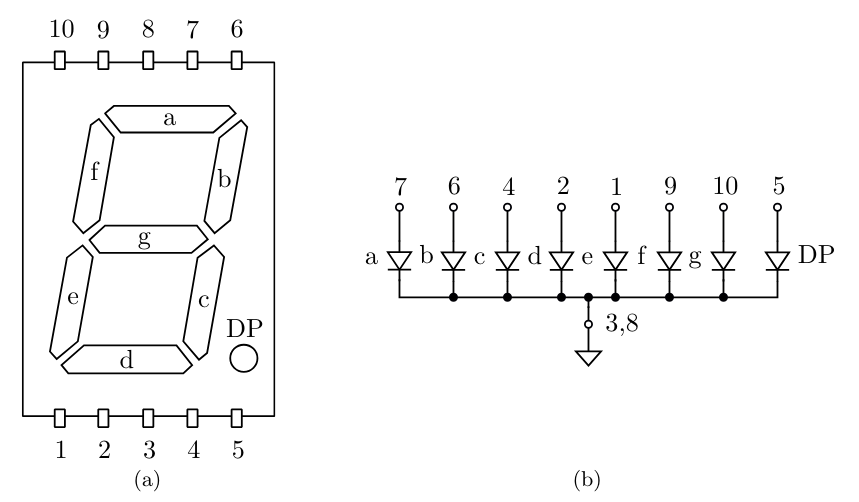
\includegraphics[width=0.5\linewidth]{images/7-segment.png}
    \caption{7-Segment Anzeige}
    \label{fig:siebe-segment}
\end{figure}

\begin{table}[h]
\centering

\begin{tabular}{|c|c|c|c|c|c|c|c|c|c|}
\hline
\textbf{Ziffer} & \textbf{a} & \textbf{b} & \textbf{c} & \textbf{d} & \textbf{e} & \textbf{f} & \textbf{g} & \textbf{dp} \\ \hline
0 & 1 & 1 & 1 & 1 & 1 & 1 & 0 & 0 \\ \hline
1 & 0 & 1 & 1 & 0 & 0 & 0 & 0 & 0 \\ \hline
2 & 1 & 1 & 0 & 1 & 1 & 0 & 1 & 0 \\ \hline
3 & 1 & 1 & 1 & 1 & 0 & 0 & 1 & 0 \\ \hline
4 & 0 & 1 & 1 & 0 & 0 & 1 & 1 & 0 \\ \hline
5 & 1 & 0 & 1 & 1 & 0 & 1 & 1 & 0 \\ \hline
6 & 1 & 0 & 1 & 1 & 1 & 1 & 1 & 0 \\ \hline
7 & 1 & 1 & 1 & 0 & 0 & 0 & 0 & 0 \\ \hline
8 & 1 & 1 & 1 & 1 & 1 & 1 & 1 & 0 \\ \hline
9 & 1 & 1 & 1 & 1 & 0 & 1 & 1 & 0 \\ \hline
\end{tabular}
\caption{Segmentbelegung für 7-Segment-Anzeige (High-aktiv)}
\end{table}

\subsubsection{Berechnung Vorwiderstände}
Die Benötigte DiodenSpannung der LEDs ist $U_D=2V$ bei einem Strom $I_D=15mA$. Es ist mit einer Spannung von $U_{CC}=5V$ an den Ausgängen des Schieberegisters zu rechnen. Der Vorwiederstand Kann wie folgt berechnet werden:

$
U_{R_V} = U_{CC} - U_D = 5V - 2V = 3V
$

$
I_{R_V} = I_D = 15mA
$

$
R_V=\frac{U_{R_V}}{I_{R_V}} = \frac{3V}{15mA} = 200 \Omega
$

Die E6 Reihe enthält die Werte (1,0 1,5 2,2 3,3 4,7 6,8). Damit sind die nähesten 2 Widerstände $150\Omega$ und $220\Omega$. Da der Strom von $I_D=15mA$ nicht überschritten werden soll, wählen wir den größeren Widerstand. Somit ist der Vorwiderstand: $R_V=220\Omega$

\subsection{Praktikumsaufgabe}

\subsubsection{7 Segment}

\subsection{b}


\subsubsection{c}

\begin{minted}{c++}
// C++ code
//
const int SHIFT_IN=4;
const int SHIFT_OUTPUT=5;
const int SHIFT_CLK=6;

const int BUTTON_UP = 2;
const int BUTTON_DOWN = 3;

volatile int currentNumber = 0;
volatile bool needsUpdate = true;

unsigned long lastInterruptTime = 0;
const unsigned long debounceDelay = 200;

const uint8_t segmentPatterns[] = {
  0b11111100, // 0
  0b01100000, // 1
  0b11011010, // 2
  0b11110010, // 3
  0b01100110, // 4
  0b10110110, // 5
  0b10111110, // 6
  0b11100000, // 7
  0b11111110, // 8
  0b11110110  // 9
};

void setup()
{
  pinMode(LED_BUILTIN, OUTPUT);
  
  pinMode(SHIFT_IN, OUTPUT);
  pinMode(SHIFT_CLK, OUTPUT);
  pinMode(SHIFT_OUTPUT, OUTPUT);
  
  pinMode(BUTTON_UP, INPUT_PULLUP);
  pinMode(BUTTON_DOWN, INPUT_PULLUP);
  
  attachInterrupt(digitalPinToInterrupt(BUTTON_UP), countUp, FALLING);
  attachInterrupt(digitalPinToInterrupt(BUTTON_DOWN), countDown, FALLING);
}
  
void loop()
{
  if(needsUpdate) {
    needsUpdate = false;
    setShiftRegister(currentNumber);
  }
}

void countUp() {
  unsigned long time = millis();
  if (time - lastInterruptTime > debounceDelay) {
    if(currentNumber >= 9) {
      currentNumber = 0;
    } else {
      currentNumber++; 
    }
    needsUpdate = true;
  }
  lastInterruptTime = time;
}

void countDown() {
  unsigned long time = millis();
  if (time - lastInterruptTime > debounceDelay) {
    if(currentNumber <=0) {
      currentNumber = 9;
    } else {
      currentNumber--; 
    }
    needsUpdate = true;
  }
  lastInterruptTime = time;
}


void setShiftRegister(int number) {
  digitalWrite(SHIFT_OUTPUT, LOW);
  
  shiftOut(SHIFT_IN, SHIFT_CLK, LSBFIRST, segmentPatterns[number]);
  
  digitalWrite(SHIFT_OUTPUT, HIGH);
}

\end{minted}

\subsubsection{d} 

\begin{minted}{c++}
    
// C++ code
//
const int SHIFT_IN=4;
const int SHIFT_OUTPUT=5;
const int SHIFT_CLK=6;

const int BUTTON_UP = 2;
const int BUTTON_DOWN = 3;

volatile int currentNumber = 0;
volatile bool needsUpdate = true;

unsigned long lastInterruptTime = 0;
const unsigned long debounceDelay = 200;


const int MOTOR_LED_OFF=9;
const int MOTOR_LED_ON=8;
const int MOTOR_PWM_LEFT=10;

volatile int motorSpeed = 0;

const uint8_t segmentPatterns[] = {
  0b11111100, // 0
  0b01100000, // 1
  0b11011010, // 2
  0b11110010, // 3
  0b01100110, // 4
  0b10110110, // 5
  0b10111110, // 6
  0b11100000, // 7
  0b11111110, // 8
  0b11110110  // 9
};

void setup()
{
  pinMode(LED_BUILTIN, OUTPUT);
  
  pinMode(SHIFT_IN, OUTPUT);
  pinMode(SHIFT_CLK, OUTPUT);
  pinMode(SHIFT_OUTPUT, OUTPUT);
  
  pinMode(MOTOR_PWM_LEFT, OUTPUT);
  pinMode(MOTOR_LED_OFF, OUTPUT);
  pinMode(MOTOR_PWM_LEFT, OUTPUT);
  
  pinMode(BUTTON_UP, INPUT_PULLUP);
  pinMode(MOTOR_LED_ON, OUTPUT);
  
  attachInterrupt(digitalPinToInterrupt(BUTTON_UP), countUp, FALLING);
  attachInterrupt(digitalPinToInterrupt(BUTTON_DOWN), countDown, FALLING);

  
  
  setShiftRegister(currentNumber);
  setMotorSpeed(currentNumber);
}
  
void loop()
{
  if(needsUpdate) {
    needsUpdate = false;
    setShiftRegister(currentNumber);
    setMotorSpeed(currentNumber);
  }
}

void countUp() {
  unsigned long time = millis();
  if (time - lastInterruptTime > debounceDelay) {
    if(currentNumber >= 9) {
      currentNumber = 0   ;
    } else {
      currentNumber++; 
    }
    needsUpdate = true;
  }
  lastInterruptTime = time;
}

void countDown() {
  unsigned long time = millis();
  if (time - lastInterruptTime > debounceDelay) {
    if(currentNumber <=0) {
      currentNumber = 9;
    } else {
      currentNumber--; 
    }
    needsUpdate = true;
  }
  lastInterruptTime = time;
}


void setShiftRegister(int number) {
  digitalWrite(SHIFT_OUTPUT, LOW);
  
  shiftOut(SHIFT_IN, SHIFT_CLK, LSBFIRST, segmentPatterns[number]);
  
  digitalWrite(SHIFT_OUTPUT, HIGH);
}

void setMotorSpeed(int number) {
  int pwmValue = map(number, 0, 9, 0, 255);
  analogWrite(MOTOR_PWM_LEFT, pwmValue);
  
  if(number != 0) {
    digitalWrite(MOTOR_LED_OFF, LOW);
    digitalWrite(MOTOR_LED_ON, HIGH);
  } else {
    digitalWrite(MOTOR_LED_ON, LOW);
    digitalWrite(MOTOR_LED_OFF, HIGH);
  }
}
\end{minted}

\subsubsection{e}

\begin{minted}{c++}
// C++ code
//
const int SHIFT_IN=4;
const int SHIFT_OUTPUT=5;
const int SHIFT_CLK=6;

const int BUTTON_UP = 2;
const int BUTTON_DOWN = 3;

volatile int currentNumber = 0;
volatile bool needsUpdate = true;

unsigned long lastInterruptTime = 0;
const unsigned long debounceDelay = 200;


const int MOTOR_LED_OFF=9;
const int MOTOR_LED_ON=8;
const int MOTOR_PWM_LEFT=10;

volatile int motorSpeed = 0;

const int SENSOR_TRIGGER = 13;
const int SENSOR_ECHO = 12;

unsigned long lastSensorTime = 0;
unsigned long sensorPeriodMillis = 60;

  
const uint8_t segmentPatterns[] = {
  0b11111100, // 0
  0b01100000, // 1
  0b11011010, // 2
  0b11110010, // 3
  0b01100110, // 4
  0b10110110, // 5
  0b10111110, // 6
  0b11100000, // 7
  0b11111110, // 8
  0b11110110  // 9
};

void setup()
{
  Serial.begin(9600);
  
  pinMode(LED_BUILTIN, OUTPUT);
  
  pinMode(SHIFT_IN, OUTPUT);
  pinMode(SHIFT_CLK, OUTPUT);
  pinMode(SHIFT_OUTPUT, OUTPUT);
  
  pinMode(MOTOR_PWM_LEFT, OUTPUT);
  pinMode(MOTOR_LED_OFF, OUTPUT);
  pinMode(MOTOR_PWM_LEFT, OUTPUT);
  
  pinMode(MOTOR_LED_OFF, OUTPUT);
  pinMode(MOTOR_PWM_LEFT, OUTPUT);
  
  pinMode(BUTTON_UP, INPUT_PULLUP);
  pinMode(MOTOR_LED_ON, OUTPUT);
  
  attachInterrupt(digitalPinToInterrupt(BUTTON_UP), countUp, FALLING);
  attachInterrupt(digitalPinToInterrupt(BUTTON_DOWN), countDown, FALLING);

  pinMode(SENSOR_TRIGGER, OUTPUT);
  pinMode(SENSOR_ECHO, INPUT);
  
  setShiftRegister(currentNumber);
  setMotorSpeed(currentNumber);
  digitalWrite(SENSOR_TRIGGER, HIGH);
}
  
void loop()
{
  if(needsUpdate) {
    needsUpdate = false;
    setShiftRegister(currentNumber);
    setMotorSpeed(currentNumber);
  }
  
  unsigned long time = millis();
  if(time - sensorPeriodMillis > lastSensorTime) {
    float distance = getDistance();
    Serial.print(distance);
  	Serial.println(" cm");
    lastSensorTime = time;
  }
}

void countUp() {
  unsigned long time = millis();
  if (time - lastInterruptTime > debounceDelay) {
    if(currentNumber >= 9) {
      currentNumber = 0   ;
    } else {
      currentNumber++; 
    }
    needsUpdate = true;
  }
  lastInterruptTime = time;
}

void countDown() {
  unsigned long = millis();
  if (time - lastInterruptTime > debounceDelay) {
    if(currentNumber <=0) {
      currentNumber = 9;
    } else {
      currentNumber--; 
    }
    needsUpdate = true;
  }
  lastInterruptTime = time;
}


void setShiftRegister(int number) {
  digitalWrite(SHIFT_OUTPUT, LOW);
  
  shiftOut(SHIFT_IN, SHIFT_CLK, LSBFIRST, segmentPatterns[number]);
  
  digitalWrite(SHIFT_OUTPUT, HIGH);
}

void setMotorSpeed(int number) {
  int pwmValue = map(number, 0, 9, 0, 255);
  analogWrite(MOTOR_PWM_LEFT, pwmValue);
  
  if(number != 0) {
    digitalWrite(MOTOR_LED_OFF, LOW);
    digitalWrite(MOTOR_LED_ON, HIGH);
  } else {
    digitalWrite(MOTOR_LED_ON, LOW);
    digitalWrite(MOTOR_LED_OFF, HIGH);
  }
}

float getDistance() {
  digitalWrite(SENSOR_TRIGGER, LOW);
  delayMicroseconds(20);
    
  long duration = pulseIn(SENSOR_ECHO, HIGH, 200000);
  if (duration <= 0) duration = 200000;  
  float distance = (duration * 0.0343) / 2;
  
  digitalWrite(SENSOR_TRIGGER, HIGH);
  return distance;
}
\end{minted}


